\documentclass[UTF8,a4paper]{ctexart}
\usepackage[margin=1in]{geometry}
\usepackage{fancyhdr,hyperref,float,graphicx,color}
\pagestyle{fancy}
\hypersetup{hidelinks}

\lhead{\bfseries \leftmark}
\chead{}
\rhead{SCUT}
\lfoot{\url{https://github.com/285571052}}
\cfoot{qhy}
\rfoot{\thepage}
\setlength{\headheight}{13pt}
\renewcommand{\headrulewidth}{0.4pt}
\renewcommand{\footrulewidth}{0.4pt}

\setlength{\parindent}{0pt}
\newcommand{\spaceline}{\vspace{\baselineskip}}

\author{ qhy }
\date{\today}
\title{操作系统}

\begin{document}
  \maketitle
  \tableofcontents
  \newpage

  \section{介绍}

  操作系统为童虎提供良好的用户接口

  操作系统是一个资源管理器,对多进程以及资源(共享)进行控制

  \section{进程与线程}
  {\color{blue}分三次课讲}

  \textbf{进程的创建时间:}
  \begin{itemize}
    \item 系统启动,reboot
    \item 命令行或打开图标
    \item fork(),创建子进程
    \item 启动一个批处理(batch job)
  \end{itemize}

  {\color{blue}命令行后面加个$\&$ 表示后台运行}

  \spaceline
  \textbf{进程的终止:}
  \begin{itemize}
    \item 正常退出,Normal exit\\
    end of main
    \item 错误终止 error exit\\
    exit(2)
    \item 致命错误,Fatal error\\
    除0等
    \item 被终止,kill by another process\\
    kill pid
  \end{itemize}

  \textbf{用户与程序的关系:}
  用户启动程序,有两种情况:
  \begin{itemize}
    \item 多个用户启动多个程序
    \item 多个用户共享一个实例
  \end{itemize}

  \textbf{实例:}一个实例对应一个进程 , 一个进程可以对应多个程序。

  {\color{blue}查看进程:
  \begin{itemize}
    \item Linux\\
    ps -e
    \item Windows\\
    ctrl + alt + delete
  \end{itemize}}

  \subsection{进程模型}
  主要有两种分类:
  \begin{itemize}
    \item 多进程,串行运行
    \item 多进程,并行运行\\
    实际上是多个进程交替运行一段时间,在单处理器机器上,本质上还是串行运行
    ,即某个时间点只有一个程序运行(分时运行)
  \end{itemize}

  \textbf{进程的层次结构:}父进程可以创建子进程,子进程也可以创建它的子进程。

  若一堆进程有同一个父进程,则称为进程组。

  进程的状态:
  \begin{figure}[H]
    \centering
    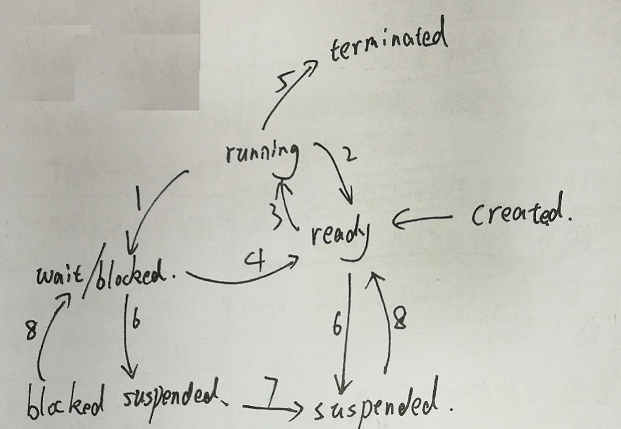
\includegraphics[scale = 0.3]{assets/caozuoxitong_fe21f.png}
    \caption{进程的状态}
  \end{figure}

  \begin{itemize}
    \item [0.] 创建进程
    \item [1.] 阻塞状态\\
    等待非CPU资源的申请,如I/O的申请
    \item [2.] 停止运行当前进程,运行其他进程
    \item [3.] 运行当前程序
    \item [4.] 一切准备就绪(申请得到资源等),等待运行(等待CPU时间分配)
    \item [5.] 进程终止
    \item [6.] 进程挂起\\
    (当内存紧张时)先把进程非运行着的进程放一边去
    \item [7.] 等待的设备已经可用,不会直接进入ready而是进入suspended
    \item [8.] 唤醒

  \end{itemize}

    \subsection{调度}
    \textbf{为什么需要调度?}\\
    当计算机系统是多道程序设计系统时,通常就会有多个进程或县城同时竞争 CPU ,只要有两个或更多的进程处于就绪
    状态,这种情形就会发生。如果只有一个CPU可用,那么久必须选择下一个要运行的进程。在操作系统中,完成选择工作
    的一部分就称为\textbf{调度程序(scheduler)},该程序使用的算法称为\textbf{调度算法(scheduling algorithm)}

    \spaceline
    \textbf{抢占式调度与非抢占式调度:}
    \begin{itemize}
      \item 抢占式调度(非当前运行着的进程控制)\\
      抢占主要体现在CPU选择下一个任务的时候,某些任务优先占有的CPU。\\
      分为两个阶段,首先是运行程序被强行中断至就绪状态(或者运行程序运行完毕或阻塞),\\
      然后优先级\footnote{优先级:这里的优先级是广义上的优先级,不一定是指一个数字什么的,也可以是其他的量}高的进程。

      \item 非抢占式调度\\
      同优先级的任务,按照某种规则进行调度。\\
      主要有两个方面,一个是是资源放弃,一个是按规则使用。\\
      程序运行到终止或阻塞时,自愿放弃对CPU的占用\\
      或者当前运行的程序CPU时间用完,被强制中断后,同优先级的处于队列首的进程接着占用CPU
    \end{itemize}

    \spaceline
    \textbf{进程的行为:}
    \begin{itemize}
      \item 长时间占有CPU-计算密集型
      \item 短时间占有CPU-I/O密集型
    \end{itemize}

    \spaceline
    \textbf{何时调度?执行调度程序的时机?}
    \begin{itemize}
      \item 进程创建/终止
      \item O/O中断
      \item 运行中的进程被阻塞
      \item 时钟中断
    \end{itemize}

    \spaceline
    \textbf{调度需要考虑的因素:}
    \begin{itemize}
      \item 公平
      \item CPU利用率
      \item 周转时间{\color{red} ????后面进行补充}
      \item 等待时间{\color{red} ????后面进行补充}
      \item 响应时间{\color{red} ????后面进行补充}
      \item 调度的策略
      \item 截止时间\\要求在截止时间内完成作业
    \end{itemize}

    \spaceline
    按照运行的环境,\textbf{主要可以划分成3类:}
    \begin{itemize}
      \item 批处理系统\\
      要求最大吞吐量,最小周转时间,同时CPU利用率高\\
      批处理系统中,每个任务都是严格按顺序执行,每个任务都是\textbf{一次性完成}\\
      即轮到任务1,只有任务1完成了之后才进行下一个任务。(基本单元是一个完整的任务)
      \item 交互式系统\\
      要求最小响应时间\\
      在实现上,把CPU划分成若干个时间片,再按一定规则对时间片进行分配。\\
      注意,按时间片执行,也就意味着,一个时间片内不一定能完成一个任务。(基本单元是一个CPU时间片)
      \item 实时系统\\
      在截止时间之前要完成作业
    \end{itemize}

    \spaceline
    \textbf{批处理系统中的调度:}
    \begin{itemize}
      \item 先来先服务\\
      先到的任务先处理,使用队列实现
      \item 最短作业优先\\
      \item 最短剩余时间优先\\
      在没有新任务的时候,这个和上一个调度室完全一样的。\\
      当新任务进入时,如果新任务的剩余时间比当前运行着的任务还要少,那么立刻挂起当前任务,
      转去执行新来的,剩余时间更少的任务
    \end{itemize}

    \spaceline
    \textbf{交互式系统}
    \begin{itemize}
      \item 转轮调度\\
      每个任务按队列顺序一次使用时间片,使用完之后进入队尾直到任务完成。\\
      时间片设得太短会导致过多的进程切换,降低了CPU的效率;而设得太长又可能引起对短的交互请求的响应时间变长。\\
      将时间片设为20ms$~$50ms通常是一个比较合理得折中。

      \item 优先级调度
      高优先级的先占用CPU\\
      为了防止高优先级进程无休止地运行下去,调度程序可以在每个时钟滴答(即每个时钟中断)降低当前进程的优先级。\\
      UNIX优先级:$pri = 40 + nice + \frac{cpu}{2}$

      \item 多级队列
      与优先级的思想类似,但是这里的优先级不是体现在优先占用CPU时间,而是不同优先级,连续占用CPU时间片的数目不一样。\\
      比如,最高级优先级的进程运行一个时间片,次高的运行2个时间片,以此类推\\
      那么如果确定优先级?\\
      一个进程初次被分配一个时间片,再次被分配两个,接着更多。\\
      (这也是为什么次高的进程反而占有的时间片更长了,因此,占用CPU的次数越多,说明这个进程需要的时间越长)\\
      除此之外,也可以通过其他姿势调整优先级。

      \item 最短进程优先{\color{red} ????后面进行补充}

      \item 保证调度\\
      保证调度考虑的因素和前面不同,这个调度是向进程作出明确的性能保证。即如果进程是等价的,那么要保证这些进程占有的CPU时间相同\\
      由于各个进程实际获得的CPU时间是已知的,所以很容易计算出真正获得的CPU时间和应获得的CPU时间(对进程的保证)之比。\\
      比率为0.5说明一个进程只获得应得时间的一半,而比率为2.0则说明它获得应得时间的2倍。\\
      于是该算法随后转向比率最低的进程,直到该进程的比率超过它的最接近竞争者为止。

      \item 彩票调度\\
      每个进程都分配到彩票,中彩票的进程获得CPU时间。\\
      可以通过控制进程获得的彩票的数目来控制占用CPU时间的比例。\\
      还有其他玩法,对于协同进程可以集合彩票一起用\\
      比如A必须等待B进程完成才能继续,A可以把票给B使得B能更多占有CPU时间

      \item 公平分享调度\\
      和保证调度的思想有点类似,不过公平分享调度是针对用户而非进程。\\
      前面的调度都是针对进程而言的,如果用户1启动9个进程,而用户2启动了一个进程。\\
      这样用户1得到90\%的CPU时间,而用户2得到了10\%的CPU时间,显然是不公平的。\\
      为了避免这种情况,某些系统在调度处理之前考虑谁拥有进程这一因素,在这种模式中,
      每个用户分配到CPU时间的一部分,而调度程序以一种强制的方式选择进程。\\
      比如前2个CPU时间片给用户1的进程,后2个CPU时间片给用户2的进程。\\
      当然也可以使用类似保证调度的思想,这取决于对\textbf{公平}的含义。

    \end{itemize}

    注:可以使用\textbf{平均等待时间}来衡量每个调度的优劣

    \spaceline
    \textbf{多CPU的调度:}
    \begin{itemize}
      \item 自调用\\
      每个CPU有自己的调度队列,任务分配到哪个CPU就在哪个CPU上运行。
      \item 主从式调度\\
      一个CPU运行调度程序控制其他CPU的调度,其他CPU运行被分配的任务。
      \item 非对称式\\
      某些CPU专门做某个单一的工作。\\
      比叡一个CPU专门处理网络,其他CPU处理其他任务。
      \item Gang调度\\
      对进程进行分组,以组为单位进行调度。\\
      组内的一个进程被挂起,组内的其他进程也终止。\\
      比如,send和receive两个进程,如果send被挂起不再发送,那么receive进程也没必要继续运行。
    \end{itemize}

    \spaceline
    \textbf{优先级倒置:}在调度的时候可能会出现优先级倒置的现象,比如优先级高的进程需要访问或修改内核的某些数据,\\
    而这些数据又恰巧被优先级低的进程占用而无法使用,那么优先级高的进程就需要等待优先级低的进程完成之后才能继续任务。
    这就导致优先级高的进程受制于优先级低的进程,优先级实际上并不起作用。

    \textbf{解决办法:优先级继承}:优先级低的进程继承高优先级进程的优先级,直到高优先级进程完成任务。

    \spaceline
    \textbf{实时系统:}\\
    实时系统通常可以分为\textbf{硬实时}和\textbf{软实时},前者的含义是必须满足绝对的截止时间,
    后者的含义是虽然不希望偶尔错失截止时间,但是可以容忍。

    {\color{red}后面补上可调度的定义}

    \spaceline
    \textbf{策略与机制}:调度机制位于内核,而调度策略由用户进程决定。

\end{document}
